% Generated by book/tools/notebook_to_tex.py. Do not edit by hand.

\chapter[텍스트 벡터화 (TF-IDF)]{텍스트 벡터화 (TF-IDF)}

\label{ch:01}

\markboth{텍스트 벡터화 (TF-IDF)}{텍스트 벡터화 (TF-IDF)}

\chaptermeta{01_tfidf/01_tfidf.ipynb}{https://colab.research.google.com/github/yoon-gu/neuqes-101/blob/master/01_tfidf/01_tfidf.ipynb}{텍스트를 숫자 벡터로 바꾸는 첫 관문}



\index{1TF IDF@TF-IDF}

\index{1CountVectorizer@CountVectorizer}

\index{1TfidfVectorizer@TfidfVectorizer}

\index{1sparse matrix@sparse matrix}

\index{1vocabulary@vocabulary}

\index{0텍스트 벡터화@텍스트 벡터화}

\index{0단어 빈도@단어 빈도}

\index{0희귀도 가중치@희귀도 가중치}

\index{0어휘@어휘}

\index{0희소 행렬@희소 행렬}

\index{1Bag of Words@Bag of Words}

\index{1BoW@BoW}

\index{1n gram@n-gram}

\index{1token pattern@token\_pattern}

\index{1fit transform@fit\_transform}

\index{1get feature names out@get\_feature\_names\_out}

\index{1vocabulary@vocabulary\_}

\index{1max features@max\_features}

\index{1min df@min\_df}

\index{1max df@max\_df}

\index{1OOV@OOV}

\index{1out of vocabulary@out-of-vocabulary}

\index{1CSR matrix@CSR matrix}

\index{1dense matrix@dense matrix}

\index{1load dataset@load\_dataset}

\index{1Yelp review full@Yelp review full}

\index{1pandas DataFrame@pandas DataFrame}

\index{0단어 가방@단어 가방}

\index{0엔그램@엔그램}

\index{0토큰 패턴@토큰 패턴}

\index{0어휘 사전@어휘 사전}

\index{0어휘 수@어휘 수}

\index{0어휘 밖 단어@어휘 밖 단어}

\index{0밀집 행렬@밀집 행렬}

\index{0데이터 샘플링@데이터 샘플링}



\section{변화추적표}

지금은 출발점이라 표가 한 줄뿐입니다. 장이 진행될수록 행이 누적됩니다.

\begin{booktable}{1장 변화추적표}{tab:ch01-01}
\begin{adjustbox}{max width=\textwidth}
\begin{tabular}{@{}llllll@{}}
\toprule
Ch & 모델 & 토크나이저 & Output Head & Activation & Loss \\
\midrule

\textbf{1 \(\leftarrow\) 여기} & (TF-IDF) & \inlinecode{TfidfVectorizer()} & --- & --- & --- \\
\bottomrule
\end{tabular}
\end{adjustbox}
\end{booktable}

전체 장 표는 \href{https://github.com/yoon-gu/neuqes-101\#챕터별-변화추적표}{루트 README.md}를 참고하세요.



\section{시작점에서}

이 장은 출발점입니다. 모델도 없고, 학습도 없고, loss도 없습니다. \textbf{텍스트를 숫자로 바꾸는 변환} 만 다룹니다.

왜 여기서 시작할까요? 자연어 모델은 결국 숫자 벡터를 다루는 함수입니다. BERT든 GPT든 입력 단계에서는 “텍스트 \(\to\) 숫자” 변환이 반드시 필요합니다. 가장 단순한 변환부터 손에 익혀두면, 이후 장에서 BERT의 토크나이저와 임베딩이 어떻게 다른지 비교할 기준이 생깁니다.



\section{토크나이저 노트}

이 장의 토크나이저는 \textbf{\inlinecode{CountVectorizer} / \inlinecode{TfidfVectorizer} 자체} 입니다. 따로 토크나이저 객체가 분리돼 있지 않고, 벡터라이저 한 클래스가 아래 세 가지를 동시에 합니다.

\begin{enumerate}
\def\labelenumi{\arabic{enumi}.}
\tightlist
\item
  \textbf{분리(tokenize)}: 기본은 공백·구두점 기준 단어 단위 분리. 정규식 패턴 \texttt{(?u)\textbackslash{}b\textbackslash{}w\textbackslash{}w+\textbackslash{}b}(영숫자 2자 이상)이 기본값.
\item
  \textbf{어휘 학습(vocabulary)}: 학습 데이터에 등장한 토큰을 모두 모아 정수 인덱스로 매핑.
\item
  \textbf{OOV 처리}: 학습 어휘에 없는 단어는 단순히 \textbf{무시}합니다 (BERT의 \texttt{{[}UNK{]}}처럼 별도 토큰으로 보존하지 않음).
\end{enumerate}

조금 뒤 같은 문장 \inlinecode{"I\ love\ using\ Hugging\ Face!"} 가 어떻게 토큰화되는지 직접 확인합니다.

\begin{previewBox}{미리보기}
\textbf{다음 장(\ref{ch:02}장)}: 같은 \inlinecode{TfidfVectorizer}를 그대로 사용. 토크나이저는 변하지 않습니다.
\end{previewBox}



\section{실습: Yelp 리뷰 데이터 살펴보기}

\inlinecode{yelp\_review\_full}은 Yelp 식당 리뷰 65만 건에 1-5점 별점이 달린 데이터셋입니다 (라벨은 0-4로 저장됨). 학습 흐름을 가볍게 유지하기 위해 \textbf{5,000건만 무작위 샘플링} 합니다.



\compactCodeOmitted{숫자 결과를 그림으로 확인하는 단계}

\begin{bookfigurelabel}[H]{Yelp 5,000건 샘플의 별점 분포}{fig:ch01-star-distribution}
\centering
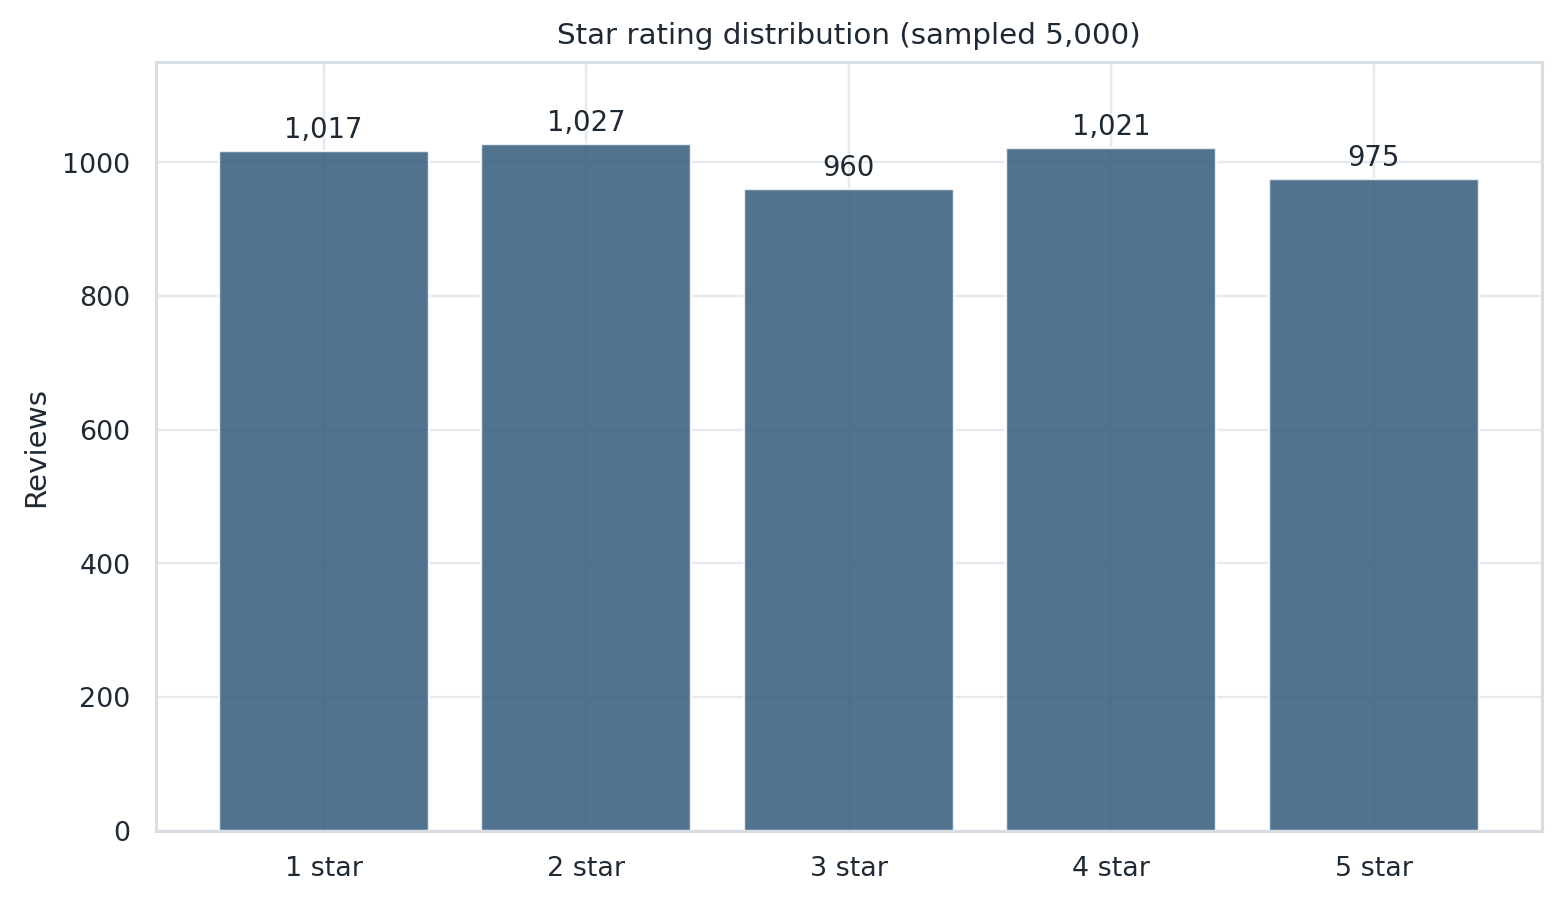
\includegraphics[width=0.72\linewidth]{assets/figures/ch01_star_distribution.png}
\end{bookfigurelabel}

\textbf{그림 읽기} --- 그림~\ref{fig:ch01-star-distribution}에서 다음 내용을 확인합니다: Yelp 5,000건 샘플의 별점 분포. 실행된 노트북에서 저장된 최신 plot 출력이므로, 코드에서 계산한 값이 어떤 평가 지점으로 이어지는지 바로 확인할 수 있습니다.



\Needspace{5\baselineskip}
\begin{lstlisting}
df["len_words"] = df["text"].str.split().str.len()
df[["len_words"]].describe()
\end{lstlisting}

\begin{codeRead}
\textbf{1행}의 \inlinecode{df["len\_words"] = df["tex...}에서는 이후 분석에서 사용할 값을 준비합니다. \textbf{2행}의 \inlinecode{df[["len\_words"]].describe()}에서는 앞 단계에서 만든 값을 바탕으로 다음 계산을 수행합니다.
\end{codeRead}

\noindent\textbf{출력.}
\begin{bookoutputbox}
len_words
count  5000.000000
mean    133.811400
std     119.787704
min       1.000000
25%      53.000000
50%     100.000000
75%     177.000000
max     977.000000
\end{bookoutputbox}
\par\vspace{0.9em}



\section{해부: CountVectorizer --- 텍스트를 “단어 횟수”로}

\inlinecode{CountVectorizer}는 가장 단순한 변환입니다.

\begin{quote}
“이 문서에 단어 X가 몇 번 나왔는가?”
\end{quote}

각 문서가 길이 V짜리 벡터로 변환됩니다 (V는 어휘 수). 대부분의 칸은 0이라 \textbf{희소(sparse)} 행렬로 저장합니다.



\Needspace{11\baselineskip}
\begin{lstlisting}
cv = CountVectorizer(max_features=10000)
X_count = cv.fit_transform(df["text"])

print(f"shape: {X_count.shape}  (n_docs, vocab_size)")
print(f"non-zero entries: {X_count.nnz:,}")
print(
    f"total cells: "
    f"{X_count.shape[0] * X_count.shape[1]:,}"
)
sparsity = 1 - X_count.nnz / (X_count.shape[0] * X_count.shape[1])
print(
    f"sparsity: "
    f"{sparsity:.2%}  (fraction of empty cells)"
)
\end{lstlisting}

\begin{codeRead}
\textbf{1행}의 \inlinecode{cv = ...}에서는 단어 횟수 기반 벡터라이저를 만듭니다. \textbf{2행}의 \inlinecode{X\_count = ...}에서는 텍스트나 라벨을 모델이 처리할 수 있는 수치 표현으로 변환합니다. \textbf{10행}의 \inlinecode{sparsity = ...}에서는 행렬에서 0인 원소의 비율을 계산합니다.
\end{codeRead}

\noindent\textbf{출력.}
\begin{bookoutputbox}
shape: (5000, 10000)  (n_docs, vocab_size)
non-zero entries: 405,803
total cells: 50,000,000
sparsity: 99.19%  (fraction of empty cells)
\end{bookoutputbox}
\par\vspace{0.9em}



\Needspace{6\baselineskip}
\begin{lstlisting}
sample = "I love using Hugging Face!"
analyzer = cv.build_analyzer()
print(f"Input sentence: {sample!r}")
print(f"Tokenized: {analyzer(sample)}")
\end{lstlisting}

\begin{codeRead}
\textbf{1행}의 \inlinecode{sample = ...}에서는 토큰화 예제로 사용할 문장을 정합니다. \textbf{2행}의 \inlinecode{analyzer = ...}에서는 벡터라이저 내부의 토큰화 규칙을 직접 호출할 함수로 꺼냅니다.
\end{codeRead}

\noindent\textbf{출력.}
\begin{bookoutputbox}
Input sentence: 'I love using Hugging Face!'
Tokenized: ['love', 'using', 'hugging', 'face']
\end{bookoutputbox}
\par\vspace{0.9em}



\textbf{관찰 포인트}

\begin{itemize}
\tightlist
\item
  모두 \textbf{소문자} 로 변환됩니다 (기본 \inlinecode{lowercase=True}).
\item
  구두점 \inlinecode{!}은 사라집니다 (정규식 패턴이 영숫자만 매칭).
\item
  \inlinecode{"I"} 같은 \textbf{단일 문자도 사라집니다} (기본 \inlinecode{token\_pattern}은 2자 이상만 인식).
\item
  학습 어휘에 없는 단어는 OOV로 \textbf{무시}됩니다 --- BERT처럼 \texttt{{[}UNK{]}}로 보존하지 않습니다.
\end{itemize}



\section{변형: TfidfVectorizer --- 흔한 단어의 영향력 줄이기}

\inlinecode{CountVectorizer}의 한계: \inlinecode{"the"}, \inlinecode{"and"} 같은 단어가 모든 리뷰에 많이 등장하니 횟수만으로는 문서 사이 차이를 잘 드러내지 못합니다.

\textbf{TF-IDF}는 두 항을 곱해 이 문제를 다룹니다.

\begin{equation}
\label{eq:ch01-01}
\text{tfidf}(t, d) = \underbrace{\text{tf}(t, d)}_{\text{문서 } d \text{에서 } t \text{의 빈도}} \cdot \underbrace{\log\frac{1 + N}{1 + \text{df}(t)}}_{\text{희귀도 가중치 (IDF)}}
\end{equation}

식~\eqref{eq:ch01-01}은 단어 빈도와 희귀도 가중치를 결합한 TF-IDF의 정의입니다.

\begin{itemize}
\tightlist
\item
  \inlinecode{tf}: 한 문서에서 단어가 얼마나 자주 나왔는가
\item
  \inlinecode{idf}: 그 단어가 \textbf{얼마나 적은 문서에 등장했는가} (모든 문서에 흔할수록 0에 가까워짐)
\end{itemize}

직관: “이 단어가 이 문서에서 자주 나오면서 동시에 다른 문서엔 흔하지 않다면, 이 문서를 특징짓는 단어”라는 가중치입니다.



\Needspace{5\baselineskip}
\begin{lstlisting}
tfidf = TfidfVectorizer(max_features=10000)
X_tfidf = tfidf.fit_transform(df["text"])
print(f"shape: {X_tfidf.shape}")
\end{lstlisting}

\noindent\textbf{출력.}
\begin{bookoutputbox}
shape: (5000, 10000)
\end{bookoutputbox}
\par\vspace{0.9em}



\textbf{관찰}: 단순 횟수 기준 top 10에는 \inlinecode{the}, \inlinecode{and} 같은 흔한 단어가 위로 올라옵니다. TF-IDF 정렬에서는 그 문서를 특징짓는 명사·형용사가 상위로 올라오는 경향을 볼 수 있습니다.

\begin{quote}
\textbf{후속 논점}: 두 방식 모두 단어를 \emph{서로 독립} 으로 취급합니다. \inlinecode{"not\ bad"}(좋다는 뜻)와 \inlinecode{"bad"}(나쁘다는 뜻)을 구분하지 못합니다. BERT가 등장하는 Phase 1에서 이 한계가 어떻게 깨지는지 확인하게 됩니다.
\end{quote}



\section{이 장에 등장한 라이브러리}

\begin{booktable}{1장 새로 등장한 라이브러리}{tab:ch01-02}
\begin{adjustbox}{max width=\textwidth}
\begin{tabular}{@{}lll@{}}
\toprule
이름 & 한 줄 설명 & 다음 장에서 \\
\midrule

\inlinecode{datasets} & Hugging Face의 데이터셋 로딩 라이브러리 (Apache Arrow 기반) & \ref{ch:07}장에서 깊게 본다 \\
\inlinecode{sklearn.feature\_extraction.text.CountVectorizer} & 횟수 벡터화 & 이후 장의 비교 기준 \\
\inlinecode{sklearn.feature\_extraction.text.TfidfVectorizer} & TF-IDF 벡터화 & \ref{ch:02}--\ref{ch:05}장에서 입력으로 계속 사용 \\
\bottomrule
\end{tabular}
\end{adjustbox}
\end{booktable}



\section{체크포인트 질문}

\begin{enumerate}
\def\labelenumi{\arabic{enumi}.}
\tightlist
\item
  \inlinecode{CountVectorizer.fit\_transform(...)}이 만든 행렬의 shape가 \inlinecode{(N,\ V)}일 때, N과 V는 각각 무엇을 의미하나요?
\item
  sparsity가 99\%를 넘는 이유는 무엇인가요?
\item
  TF-IDF가 단순 횟수보다 “문서를 특징짓는 단어”를 더 잘 뽑아내는 이유는 IDF의 어느 부분에서 오나요?
\item
  \inlinecode{CountVectorizer}가 학습 어휘에 없는 단어를 만났을 때 어떻게 처리하나요? BERT의 처리 방식과는 무엇이 다른가요?
\end{enumerate}



\section{FAQ}

\begin{faqBox}{Q1. (실무) Yelp 데이터가 너무 커서 메모리에 안 올라가는데 어떻게 하나요?}

\inlinecode{datasets}는 Apache Arrow 메모리맵을 사용해서 65만 건 전체를 RAM에 올리지 않습니다. 인덱싱 시점에만 디스크에서 읽어 옵니다. 그래서 위 셀에서 \texttt{dataset{[}“train”{]}}을 가져와도 메모리는 거의 늘어나지 않습니다.

그래도 다운스트림(예: pandas 변환, sklearn fit) 단계에서 메모리가 부담되면 두 가지를 씁니다.

\Needspace{11\baselineskip}
\begin{lstlisting}
ds = dataset["train"].shuffle(seed=42).select(range(5000))

stream = load_dataset(
    "Yelp/yelp_review_full",
    split="train",
    streaming=True,
)
for i, ex in enumerate(stream):
    if i >= 5000: break
    ...
\end{lstlisting}

\end{faqBox}

\begin{faqBox}{Q2. (실무) \inlinecode{CountVectorizer}와 \inlinecode{TfidfVectorizer} 중 뭘 써야 하나요?}

분류·검색 같은 일반 NLP 작업은 \textbf{TF-IDF가 기본 선택}입니다. 흔한 단어의 영향력을 자동으로 깎아주기 때문에 \inlinecode{LogisticRegression}, \inlinecode{LinearSVC} 같은 선형 모델과 잘 맞습니다.

\inlinecode{CountVectorizer}는 두 경우에 유리합니다.

\begin{itemize}
\tightlist
\item
  \inlinecode{MultinomialNB} (Naive Bayes): 빈도(count)를 가정한 모델이라 TF-IDF보다 Count가 더 잘 맞습니다.
\item
  “단어가 등장한 횟수 자체”가 의미 있는 분석(예: 단순 키워드 카운팅, 토픽 모델링 입력).
\end{itemize}

\end{faqBox}

\begin{faqBox}{Q3. (이론) TF-IDF의 IDF는 정확히 무슨 역할을 하나요?}

IDF(Inverse Document Frequency)는 \textbf{“이 단어가 얼마나 희귀한가”} 를 점수로 매깁니다. 식은 (sklearn 기본 옵션 기준):

\begin{equation}
\label{eq:ch01-02}
\text{idf}(t) = \log\frac{1 + N}{1 + \text{df}(t)} + 1
\end{equation}

식~\eqref{eq:ch01-02}은 문서 빈도로부터 IDF 값을 계산하는 방식입니다.

\begin{itemize}
\tightlist
\item
  \(N\): 전체 문서 수, \(\text{df}(t)\): 단어 \(t\)가 등장한 문서 수.
\item
  모든 문서에 등장하는 단어(\(\text{df}=N\)) \(\to\) \(\log 1 = 0\), 거기에 \inlinecode{+1}이 더해져 IDF는 \textbf{1}.
\item
  한 문서에만 등장 \(\to\) \(\log\frac{1+N}{2}\) 큰 값.
\end{itemize}

즉 흔한 단어는 IDF가 작아 TF-IDF 전체 값이 줄고, 드문 단어는 IDF가 커서 TF가 같아도 점수가 커집니다. “이 문서를 특징짓는 단어”를 골라내는 가중치가 IDF에서 옵니다.

\end{faqBox}

\begin{faqBox}{Q4. (이론) 어휘 수는 무엇을 기준으로 정해야 하나요? \inlinecode{max\_features=10000}은 어떻게 정한 값인가요?}

세 가지 트레이드오프가 있습니다.

\begin{enumerate}
\def\labelenumi{\arabic{enumi}.}
\tightlist
\item
  \textbf{너무 작으면}: 정보 손실. 핵심 단어가 어휘에서 잘려나감.
\item
  \textbf{너무 크면}: sparsity↑, 노이즈(오타·해시태그·고유명사 1회 등장 단어)도 같이 학습.
\item
  \textbf{모델 학습 시간/메모리}: V가 커지면 선형 모델 가중치도 V만큼 커짐.
\end{enumerate}

실무에선 보통 두 가지를 조합합니다.

\Needspace{7\baselineskip}
\begin{lstlisting}
TfidfVectorizer(
    max_features=10000,
    min_df=5,
    max_df=0.9,
)
\end{lstlisting}

5,000건짜리 영어 문서 데이터에선 5K-30K가 흔한 출발점입니다. \inlinecode{10000}은 학습 흐름을 빠르게 가져가기 위한 보수적 설정이고, 실험으로 조정하면 됩니다.

\end{faqBox}

\begin{faqBox}{Q5. (실무) sklearn에서 한국어도 처리되나요? 다음 장에서도 그대로 동작할까요?}

\textbf{기본 정규식 토크나이저로도 동작은 합니다} (한국어도 영숫자 패턴으로 잡힘). 다만 한국어는 조사 때문에 같은 어근이 다른 토큰으로 쪼개져 어휘가 폭증합니다 --- 예: \inlinecode{학교}, \inlinecode{학교는}, \inlinecode{학교가}, \inlinecode{학교를}이 전부 다른 토큰.

실무에선 형태소 분석기를 토크나이저로 끼워 넣습니다.

\Needspace{6\baselineskip}
\begin{lstlisting}
from konlpy.tag import Mecab
tokenizer = Mecab().morphs

TfidfVectorizer(tokenizer=tokenizer, token_pattern=None)
\end{lstlisting}

이 커리큘럼에서는 Phase 2(\ref{ch:15}--\ref{ch:18}장, 한국어)에서 \inlinecode{klue/bert-base}의 한국어 WordPiece 토크나이저를, Phase 3(\ref{ch:19}장부터)에서 형태소 기반 워드레벨 토크나이저를 직접 다룹니다.

\end{faqBox}

\begin{faqBox}{Q6. (이론) sparse 행렬이 dense 행렬보다 메모리에 유리한 이유는 무엇인가요? \inlinecode{.toarray()}로 바꾸면 왜 메모리가 폭발할 수 있나요?}

shape \inlinecode{(5000,\ 10000)} 행렬을 dense(\inlinecode{float64})로 만들면 \texttt{5000\ \$\textbackslash{}times\$\ 10000\ \$\textbackslash{}times\$\ 8\ byte\ \$\textbackslash{}approx\$\ 400MB}입니다. 칸 대부분이 0인데 그 0까지 다 저장합니다.

sparse(CSR) 행렬은 0이 아닌 칸만 \inlinecode{(값,\ 열\ 인덱스)}로 저장합니다. nnz가 50만이면 대략 \texttt{500000\ \$\textbackslash{}times\$\ (8\ +\ 4)\ \$\textbackslash{}approx\$\ 6MB} --- 70배 가까이 절약됩니다.

\Needspace{10\baselineskip}
\begin{lstlisting}
print(
    f"sparse nbytes $\approx$ "
    f"{(X_count.data.nbytes + X_count.indices.nbytes + X_count.indptr.nbytes) / 1e6:.1f} MB"
)
print(
    f"dense nbytes  = "
    f"{(X_count.shape[0] * X_count.shape[1] * 8) / 1e6:.1f} MB"
)
\end{lstlisting}

\inlinecode{X\_count.toarray()}를 호출하면 dense로 풀어 그 400MB짜리 배열을 메모리에 올립니다. Yelp 5,000건 정도는 버티지만, 50,000건 + max\_features 50,000으로 키우면 \texttt{50000\ \$\textbackslash{}times\$\ 50000\ \$\textbackslash{}times\$\ 8\ =\ 20GB}가 되어 Colab이 그 자리에서 중단될 수 있습니다. \textbf{sklearn 모델 대부분(LinearRegression, LogisticRegression, LinearSVC 등)은 sparse 입력을 그대로 받기 때문에 굳이 \inlinecode{.toarray()}로 바꿀 일이 없습니다.}
\end{faqBox}



\section{오류 실험 (선택)}

다음 코드를 돌려보고 결과를 비교해보세요. 어디가 달라졌나요?

\Needspace{9\baselineskip}
\begin{lstlisting}
cv2 = CountVectorizer(
    max_features=10000,
    lowercase=False,
    token_pattern=r"\b\w+\b",
)
X2 = cv2.fit_transform(df["text"])
print(len(cv2.get_feature_names_out()))
\end{lstlisting}

힌트: \inlinecode{lowercase=False}로 두면 \inlinecode{"good"}과 \inlinecode{"Good"}이 같은 토큰일까요, 다른 토큰일까요? 어휘 수가 변하는 방향을 예측해보세요.



\begin{previewBox}{미리보기: 다음 장}

\textbf{\ref{ch:02}장. 회귀 분석 (Regression \& MSE) --- 첫 모델과 손실}

\begin{itemize}
\tightlist
\item
  \inlinecode{LinearRegression}으로 별점(1-5)을 회귀합니다.
\item
  활성화 함수도 없이 출력값을 그대로 사용 --- 음수도, 5보다 큰 값도 나올 수 있습니다.
\item
  다음 장의 첫 Loss 등장: \inlinecode{MSELoss} (sklearn: squared error).
\end{itemize}
\end{previewBox}